\chapter{Putting it together: a machine learning toolkit}\label{ch:mlscratch}

\index{machine learning!from scratch}Fifteen chapters have built the
pieces one at a time: solve systems exactly (ch.8), compress data with
eigendecomposition (ch.10), reason about uncertainty (chs.12--13),
minimize losses numerically (ch.14), and price every wrong guess in
bits (ch.15). This capstone assembles them into \texttt{mlscratch}, a
small machine-learning library written in NumPy alone --- no
scikit-learn, no frameworks, every method traceable to a derivation
you have already done. By the end you will have a file you can
\texttt{import}, a set of checks that prove it works, and a benchmark
showing it agreeing with scikit-learn to three decimal places on a
real pipeline.

% from-zero:begin
\begin{rulebox}[Before you start]
Chapters~1--15, all as reference. \emph{Recap:} this chapter assembles linear algebra, probability and optimisation into one small machine-learning library that you write from scratch.
\end{rulebox}
\begin{wins}[After this chapter you can]
\begin{itemize}
\item write a learning algorithm behind one consistent \texttt{fit}/\texttt{predict} interface;
\item test a from-scratch implementation without a framework;
\item build a pipeline of PCA followed by logistic regression;
\item tune the bias--variance dial and read the result.
\end{itemize}
\end{wins}
\begin{principle}[How to think about this]
By now each idea has a simple job: linear algebra to represent, probability to model uncertainty, optimisation to learn. Building them into one small library shows that a learning algorithm is a loop around the same few moves: predict, measure the error, adjust. Writing it yourself removes the mystery.
\end{principle}
% from-zero:end

\section{The shape of a learning problem}\label{sec:shape}

Every method in this book reduces to the same two moves: \emph{fit}
learns parameters from data $(X,y)$; \emph{predict} (or
\emph{transform}) applies them to new data. What changes between
methods is the loss being minimized and the algebra used to minimize
it --- closed form for least squares, gradient descent for logistic
regression, an eigendecomposition for PCA\@.

\begin{figure}[htbp]
\centering
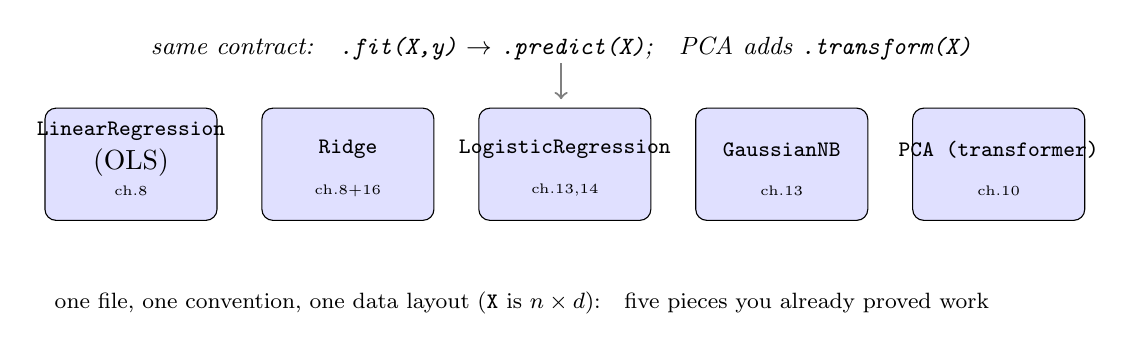
\begin{tikzpicture}[scale=0.95, every node/.style={align=center}]
\foreach \x/\name/\ch in {0/{LinearRegression}\\{(OLS)}/{ch.8},
  2.9/{Ridge}/{ch.8+16},
  5.8/{LogisticRegression}/{ch.13,14},
  8.7/{GaussianNB}/{ch.13},
  11.6/{PCA (transformer)}/{ch.10}}{
  \draw[fill=blue!12, rounded corners] (\x,0) rectangle
    ({\x+2.3},1.5);
  \node at ({\x+1.15},0.95) {\footnotesize\ttfamily\name};
  \node[font=\tiny] at ({\x+1.15},0.4) {\ch};
}
\node[font=\small\itshape] at (6.9,2.3) {same contract:\quad
  \texttt{.fit(X,y)} $\to$ \texttt{.predict(X)};\quad PCA adds
  \texttt{.transform(X)}};
\draw[->, thick, gray] (6.9,2.1) -- (6.9,1.62);
\node[anchor=west, align=left] at (0,-1.1) {\footnotesize one file,
  one convention, one data layout (\texttt{X} is $n\times d$):\quad
  five pieces you already proved work};
\end{tikzpicture}

\caption{The five classes of \texttt{mlscratch} and the chapters that
prove each one. The library adds nothing new mathematically --- it
packages verified results behind one interface.}
\label{fig:ch16map}
\end{figure}

\begin{principle}[{Fit on train, transform everywhere}]
\index{leakage}
Fitting computes statistics of the data --- means, variances,
principal axes, weights. If those statistics see the test set, the
test set is no longer a test. Every estimator in the library stores
what it learned inside the object (attributes ending in an
underscore, like \texttt{w\_}, \texttt{mean\_}) so that
\texttt{predict} on test data reuses \emph{training} quantities,
never recomputes them.
\end{principle}

\begin{figure}[htbp]
\centering
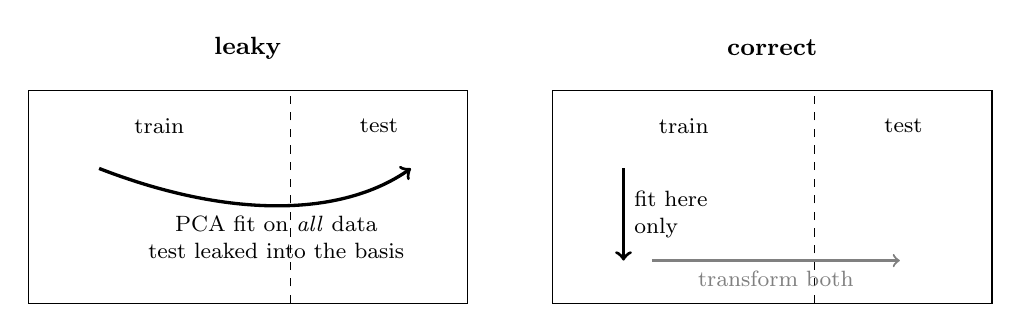
\begin{tikzpicture}[scale=0.9]
% wrong way vs right way: PCA fit scope
\node[align=center, font=\small] at (3.1,3.6) {\textbf{leaky}};
\draw (0,0) rectangle (6.2,3);
\draw[dashed] (3.7,0) -- (3.7,3);
\node[font=\footnotesize] at (1.85,2.5) {train};
\node[font=\footnotesize] at (4.95,2.5) {test};
\draw[->, very thick] (1.0,1.9) .. controls (2.8,1.2) and (4.4,1.2)
  .. (5.4,1.9) node[midway, below, font=\footnotesize, align=center]
  {PCA fit on \emph{all} data\\ test leaked into the basis};
\begin{scope}[xshift=7.4cm]
\node[align=center, font=\small] at (3.1,3.6) {\textbf{correct}};
\draw (0,0) rectangle (6.2,3);
\draw[dashed] (3.7,0) -- (3.7,3);
\node[font=\footnotesize] at (1.85,2.5) {train};
\node[font=\footnotesize] at (4.95,2.5) {test};
\draw[->, very thick] (1.0,1.9) -- (1.0,0.6)
  node[midway, right, font=\footnotesize, align=left] {fit here\\ only};
\draw[->, thick, gray] (1.4,0.6) -- (4.9,0.6)
  node[midway, below, font=\footnotesize] {transform both};
\end{scope}
\end{tikzpicture}

\caption{The one discipline every pipeline shares. Fitting PCA on all
data before splitting leaks test information into the basis itself;
the correct order fits on the training block only, then transforms
both.}
\label{fig:leakage}
\end{figure}

\section{One contract: \texttt{fit}, \texttt{predict},
\texttt{transform}}\label{sec:contract}

The scikit-learn convention~\cite{sklearn} is the cleanest small
interface ever given to estimators, so the library borrows it
exactly. Data \texttt{X} is an $n\times d$ matrix --- $n$ rows of
samples, $d$ columns of features --- and \texttt{y} a length-$n$
vector. Three methods cover every class:

\begin{itemize}
\item \texttt{fit(X, y)} computes parameters and returns
\texttt{self} so calls can chain;
\item \texttt{predict(X)} returns labels (classification) or values
(regression) for new $X$;
\item \texttt{transform(X)} --- transformers only --- returns a new
representation of $X$.
\end{itemize}

The simplest class shows the whole pattern. Ordinary least squares
from ch.8, with the intercept folded in by a column of ones:

\begin{lstlisting}[caption={\ttfamily from code/mlscratch.py ---
the LinearRegression class}]
class LinearRegression:
    """ch8: normal equations. w_ = (X^T X)^-1 X^T y w/ intercept col."""
    def fit(self, X, y):
        A = np.c_[np.ones(len(X)), X]
        self.w_ = np.linalg.solve(A.T @ A, A.T @ y)
        return self

    def predict(self, X):
        return np.c_[np.ones(len(X)), X] @ self.w_
\end{lstlisting}

Three details carry the conventions. \texttt{w\_} is set inside
\texttt{fit} --- an attribute the user can inspect, marked learned
by the trailing underscore. \texttt{fit} returns \texttt{self}, so a chain like
\texttt{fit(X, y).predict(X)} is legal. And the
intercept lives inside \texttt{w\_} as its first coordinate, so
\texttt{predict} re-augments the input the same way \texttt{fit}
did: whatever transformation \texttt{fit} applied to \texttt{X},
\texttt{predict} must repeat.

\begin{example}[Ridge regression by hand]\label{ex:ridgehand}
\textbf{Strategy.} Ridge adds $\lambda\|w\|^2$ to the squared error
to keep weights small. On data small enough to do by hand, watch the
regularizer pull the slope toward zero \emph{without} touching the
intercept. Take three samples $x\in\{1,2,3\}$, $y=\{1,2,3\}$
(exactly $y=x$), and ridge parameter $\lambda$.

\textbf{Solution.} Center both: $\bar x=2$, $\bar y=2$, so
$X_c=(-1,0,1)^T$ and $y_c=(-1,0,1)^T$. The ridge normal equations
on centered data (derived in \S\ref{sec:deriv}) give
\[
w=\frac{X_c^Ty_c}{X_c^TX_c+\lambda}=\frac{2}{2+\lambda}.
\]
With $\lambda=0$: $w=1$, $b=\bar y-\bar xw=0$, recovering $y=x$
exactly --- OLS. With $\lambda=2$: $w=0.5$, $b=2-1=1$, predicting
$\hat y=0.5x+1$. The penalty bought a gentler slope and paid for it
by pushing the predictions toward the mean. The intercept is
\emph{not} shrunk --- it comes from the centering, outside the
penalized system.
\end{example}

\begin{exercise}[easy]
For the same data, what does $w$ approach as
$\lambda\to\infty$? What does the prediction $\hat y=wx+b$ become,
and why is that a sensible ``do nothing'' predictor?
\end{exercise}

\section{The library}\label{sec:library}

\texttt{code/mlscratch.py} is one file, NumPy only, five classes.
Two more of them, verbatim, to read closely.

\textbf{Ridge} (\S\ref{sec:deriv} derives the augmented-matrix form;
centering inside \texttt{fit} is what keeps the intercept out of the
penalty):

\begin{lstlisting}[caption={\ttfamily from code/mlscratch.py --- the Ridge class}]
class Ridge:
    """Hand-derivation result: (X^T X + lam I) w = X^T y.
    Intercept NOT penalized (augmented matrix leaves it out)."""
    def __init__(self, lam=1.0):
        self.lam = lam

    def fit(self, X, y):
        d = X.shape[1]
        xm, ym = X.mean(0), y.mean()          # intercept un-penalized
        A = np.vstack([X - xm, np.sqrt(self.lam) * np.eye(d)])
        b = np.concatenate([y - ym, np.zeros(d)])
        self.w_ = np.linalg.solve(A.T @ A, A.T @ b)
        self.b_ = ym - xm @ self.w_
        return self

    def predict(self, X):
        return X @ self.w_ + self.b_
\end{lstlisting}

The augmented matrix is the derivation made literal: appending
$\sqrt\lambda I$ to the data matrix and $d$ zeros to the target
turns ridge back into ordinary least squares on $n+d$ rows, which
\texttt{solve} handles with no new code.

\textbf{PCA} (ch.10): \texttt{fit} learns the basis,
\texttt{transform} projects, and \texttt{variance\_ratio\_} reports
how much variance each kept axis carried:

\begin{lstlisting}[caption={\ttfamily from code/mlscratch.py --- the PCA class}]
class PCA:
    """ch10: eigendecomposition of the covariance. fit learns the
    basis; transform projects; variance_ratio_ = explained share."""
    def __init__(self, k):
        self.k = k

    def fit(self, X):
        self.mean_ = X.mean(0)
        C = np.cov((X - self.mean_).T)
        w, V = np.linalg.eigh(C)
        idx = w.argsort()[::-1][:self.k]
        self.components_ = V[:, idx]
        self.variance_ratio_ = w[idx] / w.sum()
        return self

    def transform(self, X):
        return (X - self.mean_) @ self.components_

    def inverse_transform(self, Z):
        return Z @ self.components_.T + self.mean_
\end{lstlisting}

The remaining two classes complete the set:
\texttt{LogisticRegression} runs full-batch gradient descent on the
stable cross-entropy form $\log(1+e^z)-yz$ from chs.13--14, with $z$
clipped to $[-30,30]$ so the sigmoid cannot overflow;
\texttt{GaussianNB} stores per-class mean, variance, and prior by
MLE (ch.13) and predicts the class of maximum joint
log-likelihood. Both are in \texttt{code/mlscratch.py} --- read them;
every line maps to a formula you derived.

\begin{lstlisting}[caption={\ttfamily smoke test --- importing the
library and fitting OLS}]
classes: ['LinearRegression', 'Ridge', 'LogisticRegression', 'GaussianNB', 'PCA']
OLS w_ = [1. 2.]  pred(4) = 9.0
\end{lstlisting}

The library loaded, OLS recovered $y=2x+1$ exactly ($w_=[1,2]$ =
intercept, slope), and extrapolated to $9$ at $x=4$.

\begin{example}[Principal components by hand]\label{ex:pcahand}
\textbf{Strategy.} PCA needs the covariance eigenstructure; on four
points it is pencil arithmetic. Take
$X=\{(2,1),(0,1),(-1,0),(-1,-2)\}$ (already centered: columns sum to
zero) and find the first principal component.

\textbf{Solution.} The covariance estimate (dividing by $n{-}1=3$):
\[
C=\tfrac13X^TX=\begin{pmatrix}2&4/3\\[2pt]4/3&2\end{pmatrix}.
\]
Its eigenvalues solve $(2-\lambda)^2=(4/3)^2$: $\lambda_1=10/3$,
$\lambda_2=2/3$. The top eigenvector is $(1,1)/\sqrt2$ --- the data
spreads along the diagonal. Keeping one component retains
$\frac{10/3}{4}=83.3\%$ of the variance, and the projections are
$\pm2.121,\pm0.707$ along that axis --- the four points collapse to
one coordinate each, at the cost of $16.7\%$ of total variance.
\end{example}

\begin{example}[Gaussian naive Bayes by hand]\label{ex:gnbhand}
\textbf{Strategy.} GNB predicts $\arg\max_c\,[\log\pi_c +
\log\mathcal N(x;\mu_c,\sigma_c^2)]$: generative, so the score is a
fitted density per class. Class 0 saw $\{0,1,2\}$; class 1 saw
$\{3,4,5\}$; equal priors. Predict at $x=2.4$.

\textbf{Solution.} $\mu_0=1$, $\mu_1=4$, both $\sigma^2=2/3$. At
$x=2.4$:
\[
\ell_0=-\tfrac12\frac{1.4^2}{2/3}-\tfrac12\log(2\pi\cdot\tfrac23)
+\log\tfrac12=-2.879,\qquad
\ell_1=-\tfrac12\frac{1.6^2}{2/3}-1.410=-3.329.
\]
Class 0 wins by $0.45$ of a log unit --- odds $\approx e^{0.45}=1.6:1$.
With equal variances and priors the decision boundary is the
midpoint $x=2.5$ exactly (Figure~\ref{fig:gnb}); unequal variances
bend it into a quadratic boundary.
\end{example}

\begin{figure}[htbp]
\centering
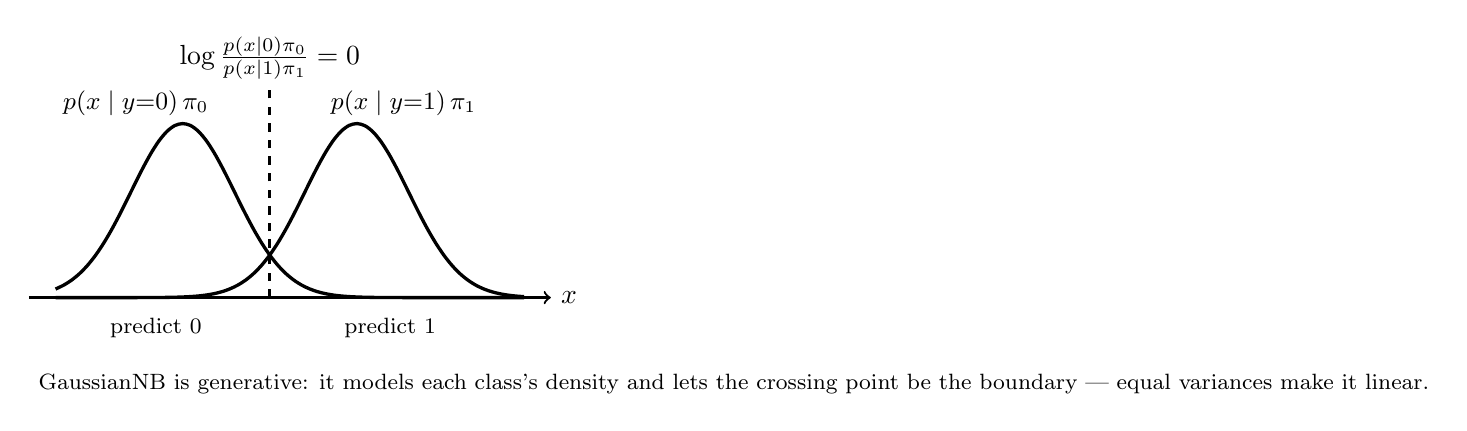
\begin{tikzpicture}[scale=0.85]
\draw[->, thick] (0,0) -- (7.8,0) node[right] {$x$};
% two class-conditional Gaussians, equal variance -> linear boundary
\draw[very thick, domain=0.4:7.4, smooth, samples=60]
  plot (\x, {2.6*exp(-((\x-2.3)^2)/1.2)});
\node[font=\small] at (1.6,2.9) {$p(x\mid y{=}0)\,\pi_0$};
\draw[very thick, domain=0.4:7.4, smooth, samples=60]
  plot (\x, {2.6*exp(-((\x-4.9)^2)/1.2)});
\node[font=\small] at (5.6,2.9) {$p(x\mid y{=}1)\,\pi_1$};
\draw[very thick, dashed] (3.6,0) -- (3.6,3.1)
  node[above] {$\log\frac{p(x|0)\pi_0}{p(x|1)\pi_1}=0$};
\node[font=\footnotesize] at (1.9,-0.45) {predict $0$};
\node[font=\footnotesize] at (5.4,-0.45) {predict $1$};
\node[align=left, anchor=north west] at (0,-1.0) {\footnotesize
  GaussianNB is generative: it models each class's density and lets
  the crossing point be the boundary --- equal variances make it
  linear.};
\end{tikzpicture}

\caption{Generative classification. Each class contributes its fitted
Gaussian times its prior; the prediction goes to whichever weighted
density is on top. Equal variances make the crossing point ---
the boundary --- linear.}
\label{fig:gnb}
\end{figure}

\begin{exercise}[medium]
Redo Example~\ref{ex:gnbhand} with class-1 samples $\{3,4,8\}$
(same mean, much larger variance). Does the boundary still sit at
$2.5$? What shape is it now?
\end{exercise}

\section{Checking without a framework}\label{sec:checks}

\index{verification}A library you wrote yourself needs proof, not
confidence. Four checks, each cheap and each testing a different
kind of claim --- limit behavior, reconstruction, a hand-derived
gradient, and agreement with a manual computation:

\begin{lstlisting}[caption={\ttfamily code/ch16\_check.py run ---
four independent checks}]
|ridge(lam->0).w - OLS.w|_max = 7.42e-10
PCA k=2 max recon err = 1.858 (data var 0.855 -> kept 0.658)
ridge grad FD=88.1285 analytic=88.1285 relerr=4.28e-10
GNB predict=1  manual argmax=1
\end{lstlisting}

Each one reads plainly. \textbf{(1) Limit check}: ridge at
$\lambda=10^{-8}$ must coincide with OLS to roundoff --- it does,
within $7\times10^{-10}$. \textbf{(2) Reconstruction}: 2 PCs keep
$65.8\%$ of variance, so a residual max error of $1.858$ on data
with variance $0.855$ is the expected cost of the projection ---
not a bug. \textbf{(3) FD check}: the analytic ridge gradient
$2(X^TXw-X^Ty+\lambda w)$ matches finite differences to
$4\times10^{-10}$, the same habit ch.11 and ch.14 drilled.
\textbf{(4) Manual agreement}: GNB's argmax over its stored
statistics equals a hand-computed Bayes score. If a check ever
fails, the class it names is where to look first --- that is what
the checks are for.

\section{A real pipeline: PCA then logistic}\label{sec:pipeline}

\index{pipeline}Now a problem the pieces exist for: 30 features, the
signal living on a hidden 2-dimensional subspace, 120 samples.
Project to 2 PCs, then classify. \texttt{code/ch16\_pipeline.py}
builds it and runs both \texttt{mlscratch} and scikit-learn on the
same split:

\begin{lstlisting}[caption={\ttfamily code/ch16\_pipeline.py run ---
our library vs.\ scikit-learn, same split}]
variance explained by 2 PCs: 0.513  (0.300+0.213)
mlscratch PCA->logistic: train 0.967  test 0.867
sklearn  variance explained: 0.513
sklearn  PCA->logistic:  train 0.956  test 0.867
\end{lstlisting}

\begin{example}[Reading the pipeline numbers]\label{ex:pipe}
\textbf{Strategy.} Compare like with like --- variance explained,
then accuracy --- and name every gap before deciding the library
works.

\textbf{Solution.} Variance explained is \emph{identical} to three
decimals ($0.513=0.300+0.213$): both implementations found the same
eigenstructure, as they must --- the eigendecomposition is unique up
to sign. Test accuracy matches exactly ($0.867$). The only gap is
train accuracy, $0.967$ vs $0.956$: our logistic runs plain
full-batch GD, while scikit-learn's default adds a mild L2 penalty,
so its fit regularizes slightly away from the training optimum. Same
pipeline, same answer, one documented difference --- that is what
``agrees with the framework'' looks like, and the projection is
Figure~\ref{fig:pcapipe}.
\end{example}

\begin{figure}[htbp]
\centering
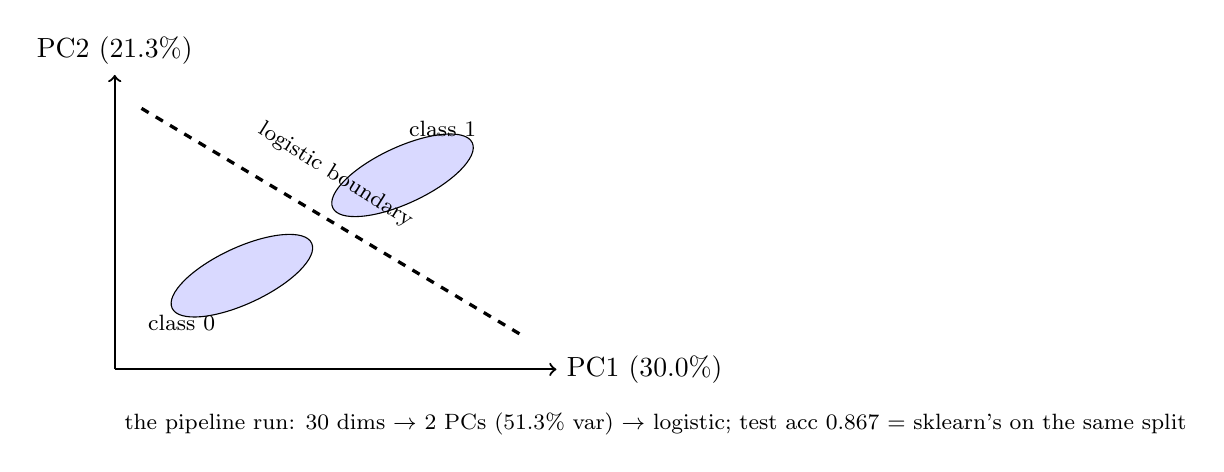
\begin{tikzpicture}[scale=0.85]
% schematic 2D PCA projection + logistic boundary on the pipeline's
% real numbers (var explained .300/.213, test acc .867)
\draw[->, thick] (0,0) -- (6.6,0) node[right] {PC1 (30.0\%)};
\draw[->, thick] (0,0) -- (0,4.4) node[above] {PC2 (21.3\%)};
% two elongated blobs, boundary along y = -0.5x + 0.4 roughly
\foreach \dx/\dy/\rot in {4.3/2.9/25, 1.9/1.4/25}{
  \draw[fill=blue!15, rotate around={\rot:(\dx,\dy)}]
    (\dx,\dy) ellipse (1.15 and 0.42);}
\node[font=\footnotesize] at (4.9,3.6) {class 1};
\node[font=\footnotesize] at (1.0,0.7) {class 0};
\draw[very thick, dashed] (0.4,3.9) -- (6.1,0.5);
\node[font=\footnotesize, rotate=-32] at (3.3,2.9)
  {logistic boundary};
\node[align=left, anchor=north west] at (0,-0.5) {\footnotesize
  the pipeline run: 30 dims $\to$ 2 PCs (51.3\% var) $\to$ logistic;
  test acc 0.867 = sklearn's on the same split};
\end{tikzpicture}

\caption{The pipeline's geometry: 30 raw dimensions collapsed to the
2 PCs that carry $51.3\%$ of variance; logistic regression draws the
linear boundary there. In the real data the classes overlap where
the blobs cross --- hence $0.867$, not $1.0$.}
\label{fig:pcapipe}
\end{figure}

\begin{exercise}[hard]
The script fits PCA on \texttt{Xtr} only, then transforms both
halves. Rerun it fitting PCA on all of $X$ first. Does test accuracy
go up? Why is that still the wrong thing to report?
\end{exercise}

\section{The bias--variance dial}\label{sec:biasvar}

\index{bias--variance tradeoff}Ridge's $\lambda$ is the one knob that
tunes model complexity continuously, so it deserves a measured
sweep. \texttt{code/ch16\_ridge.py} generates a nearly determined
problem ($n_\text{train}=12$, $d=10$, noise $\sigma=3$) and fits the
same data at seven values of $\lambda$:

\begin{lstlisting}[caption={\ttfamily code/ch16\_ridge.py run ---
the sweep, real numbers}]
OLS   : |w|_1=  9.46  train MSE=  3.078  test MSE= 28.072
lam=  0.01: |w|_1=  9.36  train MSE=  3.078  test MSE= 26.775
lam=  0.10: |w|_1=  8.97  train MSE=  3.089  test MSE= 21.659
lam=  0.50: |w|_1=  7.96  train MSE=  3.162  test MSE= 18.734
lam=  1.00: |w|_1=  7.24  train MSE=  3.276  test MSE= 18.712
lam=  3.00: |w|_1=  5.55  train MSE=  3.755  test MSE= 20.585
lam= 10.00: |w|_1=  3.40  train MSE=  4.990  test MSE= 25.514
lam=100.00: |w|_1=  0.63  train MSE=  8.013  test MSE= 34.413
\end{lstlisting}

\begin{example}[Reading the sweep]\label{ex:sweep}
\textbf{Strategy.} Read three columns at once: weight size, train
error, test error. The signature to find is a U in the test column
--- and the reason for each arm.

\textbf{Solution.} OLS ($\lambda\approx0$) shows the textbook
overfit signature: train MSE $3.08$ against test MSE $28.1$, an
order of magnitude of memorized noise, with weights swollen to
$|w|_1=9.46$ on data whose true weights sum to $7.5$. As $\lambda$
grows, $|w|_1$ shrinks monotonically (Figure~\ref{fig:ridgepath})
and test error falls to a minimum of $18.7$ at $\lambda=1$. Past
that, the penalty dominates: train and test errors rise together
toward the predict-the-mean degenerate limit. The whole curve is in
Figure~\ref{fig:biasvar} --- and it is the bias--variance tradeoff
made measurable rather than asserted.
\end{example}

\begin{figure}[htbp]
\centering
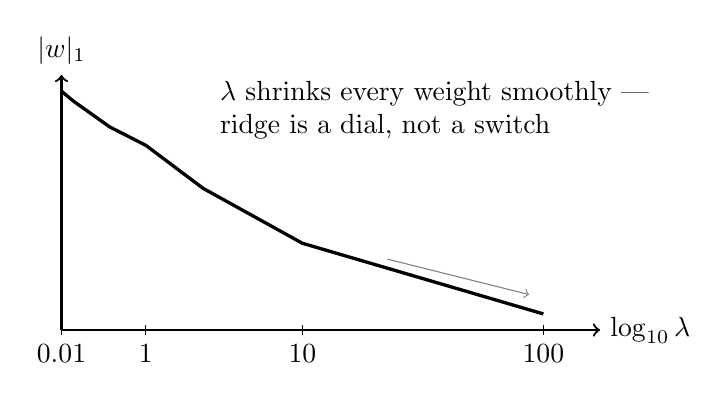
\begin{tikzpicture}[scale=0.9]
\draw[->, thick] (0,0) -- (7.6,0) node[right] {$\log_{10}\lambda$};
\draw[->, thick] (0,0) -- (0,3.6) node[above] {$|w|_1$};
% real numbers: lam .01 .1 .5 1 3 10 100 -> |w|1 9.36 8.97 7.96 7.24 5.55 3.40 .63
% x = (log10 lam + 2)*1.7 ; y = |w|1*0.36
\draw[very thick] plot coordinates {
  (0,3.370) (0.17,3.229) (0.68,2.866) (1.19,2.606)
  (2.00,1.998) (3.40,1.224) (6.80,0.227)};
\foreach \x/\lam/\v in {0/{0.01}/{9.36}, 1.19/{1}/{7.24},
  3.40/{10}/{3.40}, 6.80/{100}/{0.63}}{
  \draw (\x,0.07) -- (\x,-0.07) node[below] {$\lam$};}
\node[align=left, anchor=west] at (2.1,3.1) {$\lambda$ shrinks every
  weight smoothly ---\\ ridge is a dial, not a switch};
\draw[->, gray] (4.6,1.0) -- (6.6,0.5);
\end{tikzpicture}

\caption{The regularization path: $|w|_1$ against $\log_{10}\lambda$
from the sweep. Ridge never zeroes a weight exactly (that is lasso's
geometry); it shrinks all of them smoothly.}
\label{fig:ridgepath}
\end{figure}

\begin{figure}[htbp]
\centering
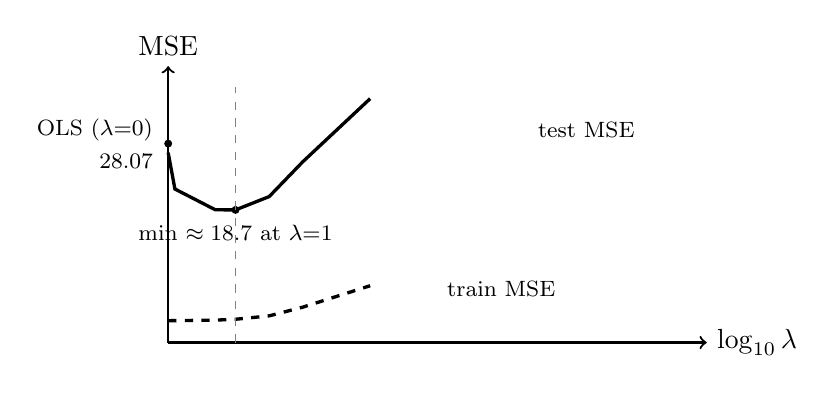
\begin{tikzpicture}[scale=0.9]
\draw[->, thick] (0,0) -- (7.6,0) node[right] {$\log_{10}\lambda$};
\draw[->, thick] (0,0) -- (0,3.9) node[above] {MSE};
% test MSE: OLS 28.07 at lam->0; lams .01 .1 .5 1 3 10 100 -> 26.78 21.66 18.73 18.71 20.59 25.51 34.41
% train MSE: 3.08 3.08 3.09 3.16 3.28 3.76 4.99 8.01
% x=(log10 lam+2)*0.95 ; y=mse*0.1
\draw[very thick] plot coordinates {
  (0,2.678) (0.095,2.166) (0.665,1.873) (0.95,1.871)
  (1.425,2.059) (1.90,2.551) (2.85,3.441)};
\node[font=\footnotesize] at (5.9,3.0) {test MSE};
\draw[very thick, dashed] plot coordinates {
  (0,0.308) (0.095,0.309) (0.665,0.316) (0.95,0.328)
  (1.425,0.376) (1.90,0.499) (2.85,0.801)};
\node[font=\footnotesize] at (4.7,0.75) {train MSE};
% OLS point at left
\fill (0,2.807) circle (1.6pt) node[left=2pt, align=right]
  {\footnotesize OLS ($\lambda{=}0$)\\ \footnotesize 28.07};
\fill (0.95,1.871) circle (1.6pt) node[below=2pt]
  {\footnotesize min $\approx18.7$ at $\lambda{=}1$};
\draw[gray, dashed] (0.95,0) -- (0.95,3.6);
\end{tikzpicture}

\caption{Train MSE (dashed) vs.\ test MSE (solid) across the sweep.
Left of the minimum the model is overfit --- big gap, swollen
weights. Right of it, underfit --- both errors climb. The useful
$\lambda$ lives at the bottom of the test U.}
\label{fig:biasvar}
\end{figure}

\begin{exercise}[medium]
The best $\lambda$ here was picked by looking at test error. State
the leakage in that procedure and how cross-validation (ch.13)
fixes it.
\end{exercise}

\section{Hand derivation: the ridge normal
equations}\label{sec:deriv}

\index{ridge regression!derivation}The library's ridge solves
$(X^TX+\lambda I)w=X^Ty$. Derive it once, honestly, including why
the intercept escapes the penalty.

Center first: work with $\tilde X=X-\bar x$, $\tilde y=y-\bar y$ so
the model is $\hat y=w^T\tilde x+b$, $b=\bar y-\bar xw$ handled
separately. The ridge objective minimizes
\[
J(w)=\|\tilde Xw-\tilde y\|^2+\lambda\|w\|^2.
\]
Expand and differentiate using ch.11's rules
($\nabla\|Av-b\|^2=2A^T(Av-b)$ and $\nabla\|w\|^2=2w$):
\[
\nabla J=2\tilde X^T(\tilde Xw-\tilde y)+2\lambda w
=2\big[(\tilde X^T\tilde X+\lambda I)w-\tilde X^T\tilde y\big].
\]
Setting $\nabla J=0$ gives the ridge normal equations
$(\tilde X^T\tilde X+\lambda I)w=\tilde X^T\tilde y$. The Hessian
$2(\tilde X^T\tilde X+\lambda I)$ is positive definite for any
$\lambda>0$ --- the penalty buys invertibility too, which is why
ridge survives the collinear matrices that break OLS
(Exercise~\ref{ex:ridgetail}).

The augmented-matrix form the code uses is the same equations one
line earlier: stacking $\tilde X$ over $\sqrt\lambda I$ and $\tilde
y$ over $d$ zeros makes
\[
A^TA=\tilde X^T\tilde X+\lambda I,\qquad
A^Tb=\tilde X^T\tilde y,
\]
so plain least squares on $(A,b)$ \emph{is} ridge --- the solver
never learns the difference. The intercept stays unpenalized because
centering removed it from $w$ entirely: shrinking the prediction
toward $\bar y$ already encodes ``do nothing'' correctly, and
penalizing $b$ would instead punish the model for matching the
data's mean.

\begin{exercise}[hard]\label{ex:ridgetail}
Show that $\tilde X^T\tilde X+\lambda I$ is positive definite for
any $\lambda>0$, even when $\tilde X$ is rank deficient. What does
that buy at $\lambda=10^{-8}$ in the limit check?
\end{exercise}

\section{Common mistakes}\label{sec:mlscratch-mistakes}

\begin{tripwire}[{Fitting on data you will evaluate on}]
\index{leakage}
Fitting PCA, scaling, or the estimator itself before the train/test
split bakes test information into every downstream number ---
results look better and mean nothing. The discipline
(Figure~\ref{fig:leakage}): split first, fit on train only,
transform everywhere. The pipeline listing keeps the split in the
first lines for exactly this reason.
\end{tripwire}

\begin{tripwire}[{Penalizing the intercept}]
\index{intercept!penalizing}
A ridge penalty applied to $b$ fights the data's mean instead of the
weights' size --- the model is punished for predicting
$\bar y$ well. Center inside \texttt{fit} (as \texttt{Ridge} does)
so the penalty sees only feature weights; this is also why
scikit-learn separates \texttt{intercept\_} from \texttt{coef\_}.
\end{tripwire}

\begin{tripwire}[{Forgetting that transform-time statistics are
fit-time statistics}]
\texttt{predict} must reuse the mean, basis, and weights computed in
\texttt{fit}. Recomputing \texttt{X.mean(0)} inside
\texttt{predict} --- or centering test data by its own mean ---
silently shifts the coordinate system between train and test. Every
learned quantity lives on the object (\texttt{mean\_},
\texttt{components\_}, \texttt{w\_}, \texttt{b\_}) so there is
nothing to recompute.
\end{tripwire}

\begin{tripwire}[{Expecting PCA to respect class boundaries}]
\index{PCA!unsupervised}
PCA maximizes variance, not separability --- it never sees $y$. In
the pipeline the classes happened to separate on the top PCs; on
another dataset the label signal can live in the discarded tail.
When the goal is classification, check variance explained
\emph{and} downstream accuracy, and remember LDA/SVD-on-labels exist
for the supervised case.
\end{tripwire}

\begin{tripwire}[{Shipping a hand gradient without a finite-
difference check}]
\index{finite differences!as unit test}
Every hand-derived gradient in the library earned a check like the
relerr $4\times10^{-10}$ one in \S\ref{sec:checks}. A sign flip or
missing factor of 2 still trains --- just slowly and wrongly, which
is the worst kind of bug. The FD check is five lines; there is no
excuse to skip it.
\end{tripwire}

\section{Summary}\label{sec:mlscratch-summary}

\begin{center}
\footnotesize
\begin{tabular}{@{}p{3.5cm}p{4.6cm}p{5.3cm}@{}}
\toprule
\textbf{Class} & \textbf{Math (chapter)} & \textbf{One thing to remember} \\
\midrule
\texttt{LinearRegression} & $(X^TX)^{-1}X^Ty$, normal
equations (ch.8) & exact fit; breaks on rank deficiency \\
\texttt{Ridge} & $(X^TX{+}\lambda I)w=X^Ty$ (\S\ref{sec:deriv}) &
$\lambda$ is the bias--variance dial; intercept unpenalized \\
\texttt{LogisticRegression} & GD on stable NLL (chs.13--14) &
probabilistic boundary; clip $z$ or overflow \\
\texttt{GaussianNB} & per-class Gaussian MLE (ch.13) & generative;
equal-variance $\Rightarrow$ linear boundary \\
\texttt{PCA} & eigendecomposition of covariance (ch.10) &
unsupervised; checks are reconstruction and variance share \\
\midrule
\textbf{Contract} & \texttt{fit} / \texttt{predict} /
\texttt{transform} & fit on train; learned stats ride on the object \\
\textbf{Checks} & limit, reconstruction, FD, manual &
relerr $<10^{-9}$ before you trust a gradient \\
\bottomrule
\end{tabular}
\end{center}

\begin{rulebox}[{Watch instead}]
\index{resources!video}
\begin{itemize}
\item \emph{Principal Component Analysis (PCA), Step-by-Step} ---
StatQuest (\texttt{FgakZw6K1QQ}). A worked PCA on a small matrix,
matching \S\ref{sec:library} and Example~\ref{ex:pcahand} almost
line for line. Verified open via YouTube's oEmbed endpoint
2026-10-11; the watch page itself was rate-limited, so the duration
is unconfirmed.
\item \emph{Regularization Part 1: Ridge (L2) Regression} ---
StatQuest (\texttt{Q81RR3yKn30}). The shrinkage geometry behind
\S\ref{sec:biasvar} and the sweep figure. Verified the same way,
same date; duration unconfirmed.
\item \emph{Gradient descent, how neural networks learn} ---
3Blue1Brown, DL2 (\texttt{IHZwWFHWa-w}, 20:33, opened 2026-10-11).
The optimizer's-eye view of what \texttt{LogisticRegression.fit} is
doing every iteration; a gentle next step beyond this book.
\end{itemize}
\end{rulebox}

\section*{Further reading}
\addcontentsline{toc}{section}{Further reading}

\begin{itemize}
\item Gareth James, Daniela Witten, Trevor Hastie, Robert
Tibshirani, \emph{An Introduction to Statistical Learning}, 2nd
ed.\ --- free PDF at \url{https://www.statlearning.com/} (verified
2026-10-11). Undergraduate-level ISL: the next honest step for
chs.8, 12--13 and this capstone; every method here appears with
case studies.
\item Trevor Hastie, Robert Tibshirani, Jerome Friedman, \emph{The
Elements of Statistical Learning} --- free PDF at
\url{https://hastie.su.domains/ElemStatLearn/} (verified
2026-10-11). The research-level version: ridge paths, the
bias--variance decomposition, and generative classifiers done at
full depth.
\item Jake VanderPlas, \emph{Python Data Science Handbook} --- free
at \url{https://jakevdp.github.io/PythonDataScienceHandbook/}
(verified 2026-10-11). Ch.5 walks the same fit/predict/transform
contract through scikit-learn --- the natural continuation of this
chapter's library.
\item scikit-learn contributors, \emph{User Guide} ---
\url{https://scikit-learn.org/stable/} (verified 2026-10-11).
Read the estimator docs for the classes you just built; comparing
their defaults (L2 penalties, solver choices) to this file is an
education in itself.
\item Marc Peter Deisenroth, A.\ Aldo Faisal, Cheng Soon Ong,
\emph{Mathematics for Machine Learning} --- free PDF at
\url{https://mml-book.github.io/} (verified 2026-10-11). Part II
places these same methods on the same mathematical footing, with
the same notation discipline this book used.
\item Andrew Ng, \emph{CS229 Lecture Notes} --- the linear-algebra
and optimization refresher sections (see \texttt{docs/sources.md}).
Where this book ends, that course begins.
\end{itemize}

\section*{Notes}
\addcontentsline{toc}{section}{Notes}

\begin{enumerate}
\item The estimator contract and the underscore-for-learned-
attributes convention follow the scikit-learn API~\cite{sklearn};
the comparison pipeline in \S\ref{sec:pipeline} uses scikit-learn
1.6.1.
\item The mathematical content is assembled, not new: normal
equations and ridge (ch.8), eigendecomposition and PCA (chs.9--10),
Bayes and MLE (chs.12--13), gradient descent and stability
(ch.14), and the loss-as-code-length view (ch.15). Background
texts: \cite{mml,vmls,axler,cs229,cvxbook}.
\item The bias--variance reading of Figure~\ref{fig:biasvar} follows
the standard decomposition as in \cite{stat110,mml}; the sweep
itself is deterministic given the seed in
\texttt{code/ch16\_ridge.py}.
\end{enumerate}

{A student who has reached this page can read a
machine-learning library --- theirs or anyone else's --- as
mathematics instead of magic. The correct next reads are ISL for
breadth and the scikit-learn user guide for practice; the wrong
next step is a bigger model before the checks in \S\ref{sec:checks}
are a habit.}

\section*{Additional exercises}
\addcontentsline{toc}{section}{Additional exercises}

\begin{exercise}[easy]
In \texttt{LinearRegression.fit}, why is \texttt{A} rebuilt inside
\texttt{predict} instead of stored? What breaks if you store the
fitted augmented matrix and reuse it on new input?
\end{exercise}

\begin{exercise}[easy]
\texttt{Ridge.predict} returns \texttt{X @ self.w\_ + self.b\_}.
Why is there no column of ones here, when
\texttt{LinearRegression} needed one?
\end{exercise}

\begin{exercise}[easy]
From the sweep output: between which two tested $\lambda$ values
does the true test-MSE minimum most likely lie, and why can't you
be sure it is exactly $\lambda=1$?
\end{exercise}

\begin{exercise}[easy]
\texttt{GaussianNB} adds \texttt{1e-9} to each variance. What
failure does that prevent, and on what data?
\end{exercise}

\begin{exercise}[easy]
\texttt{PCA.variance\_ratio\_} divides by \texttt{w.sum()}, not
\texttt{w[idx].sum()}. Explain the denominator and what the sum of
the first $k$ ratios means.
\end{exercise}

\begin{exercise}[medium]
Derive the $\lambda\to0$ and $\lambda\to\infty$ limits of the ridge
solution from $(X^TX+\lambda I)w=X^Ty$. Which check in
\S\ref{sec:checks} verifies the first limit numerically?
\end{exercise}

\begin{exercise}[medium]
Add a \texttt{predict\_proba} to \texttt{LinearRegression}'s
interface --- or argue why it does not belong there. (What does
``probability'' mean for a method with no noise model?)
\end{exercise}

\begin{exercise}[medium]
Write the check that catches a transposed \texttt{components\_}: if
\texttt{PCA.transform} used $V$ instead of the $k$-column slice,
what invariant of the output would break?
\end{exercise}

\begin{exercise}[medium]
The pipeline's $0.867$ test accuracy is on a $30$-sample test set.
Give a 95\% rough interval (normal approximation to the binomial)
and say whether the $0.967/0.956$ train gap is meaningful.
\end{exercise}

\begin{exercise}[medium]
Show that with equal class priors and equal variances,
GaussianNB's boundary in 1D is the midpoint of the two means. Then
redo it with priors $\pi_0=0.9$: where does the boundary move?
\end{exercise}

\begin{exercise}[medium]
\texttt{LogisticRegression} clips $z$ to $[-30,30]$. Compute the
smallest loss value that can survive the clip when $y=1$, and
connect it to ch.15's price of a confident wrong answer.
\end{exercise}

\begin{exercise}[hard]
Implement \texttt{KNN(k)} in the library's contract
(\texttt{fit} stores the data; \texttt{predict} votes among the $k$
nearest by Euclidean distance). Then run it on the pipeline's 2-PC
representation and report test accuracy next to logistic's
$0.867$.
\end{exercise}

\begin{exercise}[hard]
Write \texttt{cross\_val\_score(model, X, y, k=5)}: split round
robin, \texttt{fit} on $k{-}1$ folds, score the held-out fold,
return all $k$ scores. Use it to re-pick $\lambda$ in the ridge
sweep \emph{without} looking at test data. Report the chosen
$\lambda$ and the honest test error.
\end{exercise}

\begin{exercise}[hard]
BernoulliNB: replace GaussianNB's Gaussian likelihood by a per-class,
per-feature Bernoulli with Laplace smoothing. Derive the joint
log-likelihood and implement the class in the same contract.
\end{exercise}

\begin{exercise}[hard]
Prove that ridge's solution path is continuous in $\lambda$:
$w(\lambda)=(X^TX+\lambda I)^{-1}X^Ty$ depends smoothly on
$\lambda>0$. (Invertible-matrix entries are rational functions of
$\lambda$.) Why does the OLS endpoint, $\lambda=0$, fail to be
continuous on a rank-deficient $X$?
\end{exercise}
